\documentclass[../hw.tex]{subfiles}
\begin{document}
\setcounter{section}{3}
\begin{center}
  \section*{Homework 3} \label{sec:homework3}
  \subsection*{Due 2/7 9pm}
\end{center}
\addcontentsline{toc}{section}{\nameref{sec:homework3}}
\hrule \vspace{10px}

\paragraph{1.} The Center of Mass of the system is
\begin{align*}
  \vb{R} &= \frac{1}{M} \int \vb{r} \dd{m}
\end{align*}
and the mass element is the mass denisty times the volume element
\begin{align*}
  \dd{m} &= \rho \dd{V} = \frac{M}{2\pi R^2} R^2 \sin\phi \dd{\phi} \dd{\theta}
    = \frac{M}{2\pi} \sin\phi \dd{\phi} \dd{\theta}
\end{align*}
where the there is no $\dd{r}$ term because the radius is constant.
Since the center of mass is symmetric about the $x$ and $y$ axes, $X_{cm} = Y_{cm} = 0$.
The $z$ component of the center of mass is
\begin{align*}
  Z_{cm} &= \frac{1}{M} \int z \dd{m} \\
  &= \frac{1}{M} \frac{M}{2\pi} \iint z \sin\phi \dd{\phi} \dd{\theta}
\end{align*}
where $z = R \cos\phi$ so
\begin{align*}
  Z_{cm} &= \frac{R}{2\pi} \int_0^{2\pi}  \dd{\theta} \int_0^{\pi/2} \cos\phi \sin\phi \dd{\phi}  \\
  &\qusing u = \sin\phi \implies \dd{u} = \cos\phi \dd{\phi} \\
  &= \frac{R}{2\pi} [2\pi] \int_0^1 u \dd{u} \\
  Z_{cm} &= \frac{R}{2}
\end{align*}
So the COM is at $\boxed{\qt(0,0,\frac{R}{2})}$

\newpage
\paragraph*{2.}
(a) From N3L the force of the jettisoned fuel on the rocket is equal and opposite to the thrust 
on the rocket from the jettisoned fuel:
\begin{align*}
  F_{\text{fuel}} &= -F_{\text{thrust}} \\
  \dot m v_{ex} &= -\dot m v_{ex}
\end{align*}
So using N2L, the sum of the forces on the rocket is the thrust and air resistance:
\begin{align*}
  F = m \dot v = F_{\text{thrust}} - f  = - \dot m v_{ex} - bv
\end{align*}

(b) Using $\dot m = -k$
\begin{align*}
  m \dot v &= k v_{ex} - bv \\
  \frac{m}{b} \dot v &= \frac{k v_{ex}}{b} - v \\
\end{align*}
defining the constant $a = \frac{k v_{ex}}{b}$ and using separation of variables
\begin{align*}
  \frac{1}{a - v} \dd{v} &= \frac{b}{m} \dd{t} \\
\end{align*}
we can write an expression for m as a function of time through using separtion of variables again:
\begin{align*}
  \dv{m}{t} &= -k \\
  \int_{m_o}^m \dd{m}' &= -k \int_0^t \dd{t}' \\
  m - m_o &= -kt \\
  m &= m_o - kt
\end{align*}
where $m_o$ is the initial mass of the rocket. Substituting this back into main expression and 
integrating both sides:
\begin{align*}
  \int_0^v \frac{1}{a - v'} \dd{v'} &= b \int_0^t \frac{1}{m_o - kt'} \dd{t'} \\
  -\ln(a - v') \eval_0^v &= -\frac{b}{k} \ln(m_o - kt') \eval_0^t \\
  -\ln(a - v) + \ln(a) &= \frac{b}{k} \qt[-\ln(m_o - kt) + \ln(m_o)] \\
  \ln(\frac{a}{a - v}) &= \frac{b}{k} \ln(\frac{m_o}{m_o - kt})
\end{align*}
substituting back in $m = m_o - kt$ and exponentiating both sides:
\begin{align*}
  \frac{a}{a - v} &= \qt(\frac{m_o}{m})^{\frac{b}{k}} \\
  a \qt(\frac{m_o}{m})^{-\frac{b}{k}} &= a - v \\
  v &= a - a \qt(\frac{m_o}{m})^{-\frac{b}{k}} \\
  v &= a \qt[1 - \qt(\frac{m}{m_o})^{\frac{b}{k}}]
\end{align*}
subbing back in $a = \frac{k v_{ex}}{b}$ we get the final expression
\begin{align*}
  v(m) &= \frac{k v_{ex}}{b} \qt[1 - \qt(\frac{m}{m_o})^{\frac{b}{k}}]
\end{align*}

\newpage
\paragraph*{3.} \def\sectionautorefname{3} \label{hw3_3}
(a) The angular momentum vector is
\begin{align*}
  \vb*{\ell} &= \vb{r} \cross \vb{p} \\
  &= \vb{r} \cross m \dot{\vb{r}} \\
  &= m \vb{r} \cross \dot{\vb{r}}
\end{align*}
from HW 1, we know that
\begin{align*}
  \dot{\vb{r}} &= \dot r \vu{r} + r \dot\phi \vu*{\phi}
\end{align*}
so
\begin{align*}
  \vb*{\ell} &= m (r \vu{r}) \cross (\dot r \vu{r} + r \dot\phi \vu*{\phi}) \\
  &= m [r \dot r (\vu{r} \cross \vu{r}) + r (r \dot\phi) (\vu{r} \cross \vu*{\phi})] \\
  &= m [0 + r^2 \dot\phi \vu{z}] = m r^2 \omega \vu{z}
\end{align*}
where $\omega = \dot \phi$ and the magnitude of the angular momentum is
\begin{align*}
  \ell &= \abs{\vb*{\ell}} = m r^2 \omega
\end{align*}

(b) The area swept by an infinitesimal change in the planets position is equivalent to the
area of a triangle as shown in Figure 2, so
\begin{figure*}[ht]
  \centering
  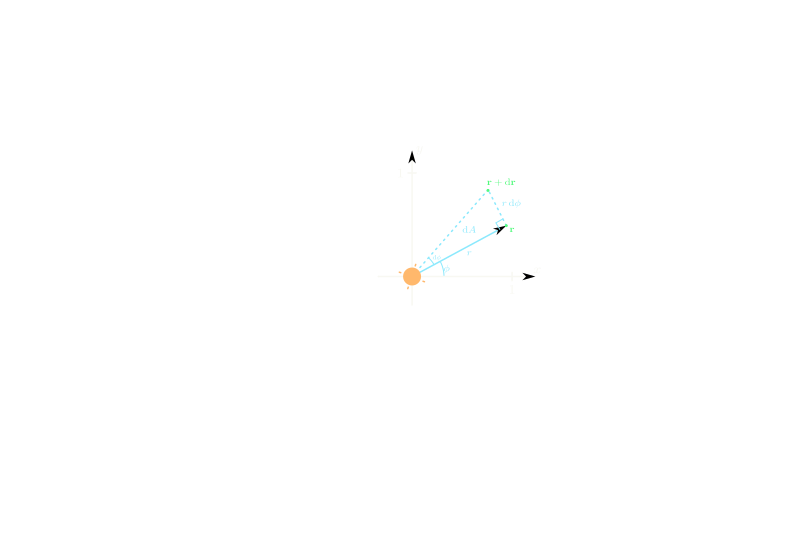
\includegraphics[width=0.4\linewidth]{hw3_3.png}
  \caption{Area swept by planet}
  \label{fig:area_swept}
\end{figure*}
\begin{align*}
  \dd{A} &= \frac{1}{2} r (r \dd{\phi}) = \frac{1}{2} r^2 \dd{\phi}
\end{align*}
dividing both sides by $\dd{t}$ gives us
\begin{align*}
  \dv{A}{t} &= \frac{1}{2} r^2 \dv{\phi}{t} = \frac{1}{2} r^2 \omega
\end{align*}
and from part (a) we know that $\ell = m r^2 \omega$ or $\omega = \frac{\ell}{m r^2}$ so
\begin{align*}
  \dv{A}{t} &= \frac{1}{2} r^2 \frac{\ell}{m r^2} = \frac{\ell}{2m}
\end{align*}
therefore, the rate in change of the area swept by the planet is a constant that is proportional 
to $\ell$.

\paragraph*{4.} $\vb{F} = -y \vu{x} + x \vu{y}$ from $P = (1,0)$ to $Q = (0,1)$

(a) For a straight line the path is given by
\begin{align*}
  y = 1 - x \qquad \dd{y} = -\dd{x}
\end{align*}
so the work done is
\begin{align*}
  W_a &= \int_P^Q F_x \dd{x} + F_y \dd{y} = \int_P^Q -y \dd{x} + x \dd{y} \\
  &= \int_{x=1}^0 -(1 - x) \dd{x} + x (-\dd{x}) \\
  &= \int_1^0 -1 \dd{x} = 1
\end{align*}

(b) For a circular path of radius 1, the path in polar coordinates is
\begin{align*}
  y &= \sin\phi \to \dd{y} = \cos\phi \dd{\phi} \\
  x &= \cos\phi \to \dd{x} = -\sin\phi \dd{\phi}
\end{align*}
from the equation of a circle $x^2 + y^2 = 1$. The limits of integration are $\phi = 0 \to \pi/2$,
and the work is
\begin{align*}
  W_b &= \int_{\phi=0}^{\pi/2} -\sin\phi(-\sin\phi) \dd{\phi} + \cos\phi \cos\phi \dd{\phi} \\
  &= \int_{\phi=0}^{\pi/2} 1 \dd{\phi} = \frac{\pi}{2}
\end{align*}

(c) Splitting this into two paths: For path 1, $y = 0$; $\dd{y} = 0$; and $x = 1 \to 0$ so
\begin{align*}
  W_1 &= \int_{x=1}^0 0 \dd{x} + x(0) = 0
\end{align*}
For path 2, $x = 0$; $\dd{x} = 0$; $y = 0 \to 1$ so
\begin{align*}
W_1 &= \int_{y=0}^1 -y(0) + 0 \dd{y} = \int_{y=0}^1 0 \dd{y} = 0
\end{align*}
And the work done is $W_c = W_1 + W_2 = 0$

(d) The force is not conservative because the work done is path dependent! We can also double check
by taking the curl:
\begin{align*}
  \curl \vb{F} &= \det \begin{vmatrix}
    \vu{x} & \vu{y} \\
    \pdv{x} & \pdv{y} \\
    -y & x
  \end{vmatrix}
  = \qt(\pdv{x} x  - \pdv{y} (-y)) \vu{z} = 2 \vu{z}
\end{align*}
which is not zero, so the force is not conservative.

\newpage
\paragraph*{5.} (a) Using the time derivatives of the polar unit vectors
\begin{align*}
  \dv{t} \vu{r} = \dot\phi \vu*{\phi} \qquad \dv{t} \vu*{\phi} = -\dot\phi \vu{r}
\end{align*}
Acceleration in polar coordinates is
\begin{align*}
  \vb{a} &= \dot{\vb{v}} = \dv{t} \dot{\vb{r}} = \dv{t} (\dot r \vu{r} + r \dot\phi \vu*{\phi}) \\
  &= \ddot r \vu r + \dot r \dot\phi \vu*\phi 
    + (\dot r \dot\phi  \vu*\phi + r \ddot \phi \vu*\phi  + r \dot\phi (-\dot\phi \vu r)) \\
  &= (\ddot r - r \dot\phi^2) \vu{r} + (r \ddot\phi + 2 \dot r \dot\phi) \vu*{\phi}
\end{align*}
so the radial and angular components of the force are 
\begin{align*}
  F_r &= m a_r = m (\ddot r - r \dot\phi^2) \\
  F_\phi &= m a_\phi = m (r \ddot\phi + 2 \dot r \dot\phi)
\end{align*}
and since the spring force is conservative with magnitude $F_s = -k(r - a) \vu{r}$ the equations of
motion are
\begin{align*}
  m(\ddot r - r \dot\phi^2) &= -k(r - a) \\
  m(r \ddot\phi + 2 \dot r \dot\phi) &= 0
\end{align*}
or
\begin{align*}
  m \ddot r - m r \dot\phi^2 + k(r - a) &= 0 \\
  r \ddot\phi + 2 \dot r \dot\phi &= 0
\end{align*}
(b) The initial angular momentum of the system is
\begin{align*}
  \ell_o = m v_o a
\end{align*}
and after some time the angular momentum is (from Problem \autoref{hw3_3})
\begin{align*}
  \ell = m r^2 \dot\phi
\end{align*}
and using the conservation of angular momentum
\begin{align*}
  \ell_o &= \ell \\
  m v_o a &= m r^2 \dot\phi \\
  \dot\phi &= \frac{v_o a}{r^2}
\end{align*}

(c) First the initial mechanical energy of the system is purely kinetic given by the initial velocity:
\begin{align*}
  E_o &= T_o = \frac{1}{2} m v_o^2
\end{align*}
the total mechanical energy of the system after some time will be the sum of the kinetic and potential
energies:
\begin{align*}
  U &= - \int_0^r \vb{F} \cdot \dd{\vb{r}}' = \int_0^r k(r - a) \dd{r}' = \frac{1}{2} k (r - a)^2 \\
  T &= \frac{1}{2} m v^2 = \frac{1}{2} m (\vb{v} \cdot \vb{v})
    = \frac{1}{2} m (\dot{\vb r} \vu{r} + r \dot\phi \vu*{\phi})
      \cdot (\dot{\vb r} \vu{r} + r \dot\phi \vu*{\phi}) 
    = \frac{1}{2} m (\dot r^2 + r^2 \dot\phi^2)
\end{align*}
And from the conservation of energy
\begin{align*}
  E_o &= E = T + U \\
  \frac{1}{2} m v_o^2 &= \frac{1}{2} m (\dot r^2 + r^2 \dot\phi^2) + \frac{1}{2} k (r - a)^2 \\
  v_o^2 &= \dot r^2 + r^2 \dot\phi^2 + \frac{k}{m} (r - a)^2
\end{align*}
substituting the result from part (b) and solving for $\dot r$:
\begin{align*}
  v_o^2 &= \dot r^2 + r^2 \qt(\frac{v_o a}{r^2})^2 + \frac{k}{m} (r - a)^2 \\
  v_o^2 &= \dot r^2 + \frac{v_o^2 a^2}{r^2} + \frac{k}{m} (r - a)^2 \\
  \dot r^2 &= v_o^2 - \frac{v_o^2 a^2}{r^2} - \frac{k}{m} (r - a)^2 \\
  \dot r &= \sqrt{v_o^2 \qt(1 - \frac{a^2}{r^2}) - \frac{k}{m} (r - a)^2}
\end{align*}

\end{document}